\documentclass{beamer}
\usetheme{Boadilla}
\usepackage{booktabs}
\usepackage{adjustbox}
\usefonttheme{serif}
\subtitle{Using Beamer}
\usepackage{pgffor}

\title{ \textbf{Stepscan Project}}
\subtitle{Results of Worksheet 1-3}
\date{\today}
\author{Saeed Kazemi}
\institute{ University of New Brunswick}
\usepackage{caption}

\begin{document}


%%%%%%%%%%%%%%%%%%%%%%%%%%%%%%%%%%%%%%%%%%%
%%%%%%%%%%%%%%%%%%%%%%%%%%%%%%%%%%%%%%%%%%%
\begin{frame}
\titlepage
\end{frame}


%%%%%%%%%%%%%%%%%%%%%%%%%%%%%%%%%%%%%%%%%%%
%%%%%%%%%%%%%%%%%%%%%%%%%%%%%%%%%%%%%%%%%%%
\begin{frame}
\frametitle{Outline}
\tableofcontents
\end{frame}


%%%%%%%%%%%%%%%%%%%%%%%%%%%%%%%%%%%%%%%%%%%
%%%%%%%%%%%%%%%%%%%%%%%%%%%%%%%%%%%%%%%%%%%
\section{Score Matrix}

\begin{frame}
\frametitle{Euclidean distance vs Correlation}
\tiny
\begin{table}
\centering
\captionsetup{labelformat=empty}
\caption{\small The accuracy of Euclidean distance and Correlation on COP features.}
\begin{tabular}{lll}
\toprule
{} &                  Accuracy Left &                 Accuracy Right \\
\midrule
Euclidean distance &  72.21 +/- 3.14 (67.67, 76.92) &  71.90 +/- 2.42 (68.69, 75.94) \\
Correlation        &  66.51 +/- 2.51 (62.50, 71.25) &  66.28 +/- 2.40 (63.09, 70.89) \\
\bottomrule
\end{tabular}

\end{table}
\begin{block}{\small Conditions}
    \footnotesize These results are average over different criteria, score matrix. Also, The PCA (keeping only 95\% variance) and z-score algorithm were applied on the all COP features.
\end{block}

\end{frame}
\begin{frame}
\frametitle{Euclidean distance vs Correlation}
\tiny
\begin{table}
\centering
\captionsetup{labelformat=empty}
\caption{\small The  ERR of different size of the test set.}
\label{tab:parameters condition}
\begin{tabular}{lll}
\toprule
{} &                  Accuracy Left &                 Accuracy Right \\
\midrule
Euclidean distance &  72.21 +/- 3.14 (67.67, 76.92) &  71.90 +/- 2.42 (68.69, 75.94) \\
Correlation        &  66.51 +/- 2.51 (62.50, 71.25) &  66.28 +/- 2.40 (63.09, 70.89) \\
\bottomrule
\end{tabular}

\end{table}
\end{frame}
\begin{frame}
\frametitle{Euclidean distance vs Correlation}
\tiny
\begin{table}
\centering
\captionsetup{labelformat=empty}
\caption{\small The number of samples in each test set.}
\label{tab:parameters condition}
\begin{tabular}{lll}
\toprule
{} &                  Accuracy Left &                 Accuracy Right \\
\midrule
Euclidean distance &  72.21 +/- 3.14 (67.67, 76.92) &  71.90 +/- 2.42 (68.69, 75.94) \\
Correlation        &  66.51 +/- 2.51 (62.50, 71.25) &  66.28 +/- 2.40 (63.09, 70.89) \\
\bottomrule
\end{tabular}

\end{table}
\end{frame}


\begin{frame}
\centering
\frametitle{Euclidean distance vs Correlation (ROC curve)}
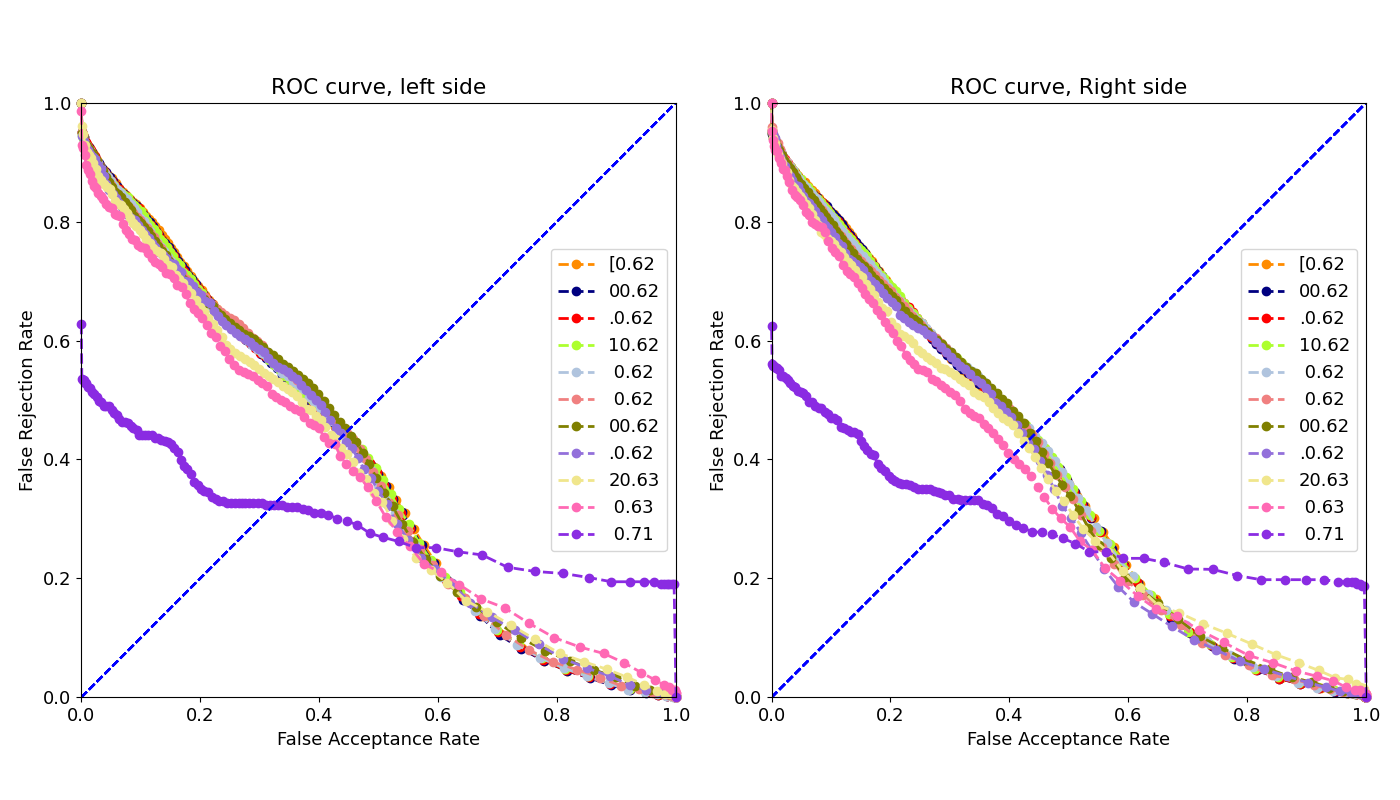
\includegraphics[scale=0.3]{Manuscripts/src/figures/testsize.png}
\end{frame}



%%%%%%%%%%%%%%%%%%%%%%%%%%%%%%%%%%%%%%%%%%%
%%%%%%%%%%%%%%%%%%%%%%%%%%%%%%%%%%%%%%%%%%%
\section{Score Matrix}

\begin{frame}
\frametitle{Euclidean distance vs Correlation}
\tiny
\begin{table}
\centering
\captionsetup{labelformat=empty}
\caption{\small The accuracy of Euclidean distance and Correlation.}
\label{tab:parameters condition}
\begin{tabular}{lrrrr}
\toprule
{} &  Accuracy Left &  Accuracy Right &  EER Left &  EER Right \\
\midrule
mean   &          79.62 &           78.23 &      0.29 &       0.31 \\
min    &          64.30 &           64.76 &      0.26 &       0.26 \\
max    &          98.87 &           98.94 &      0.36 &       0.35 \\
median &          71.26 &           68.92 &      0.29 &       0.31 \\
\bottomrule
\end{tabular}

\end{table}
\begin{table}
\centering
\captionsetup{labelformat=empty}
\caption{\small The  ERR of Euclidean distance and Correlation.}
\label{tab:parameters condition}
\begin{tabular}{lll}
\toprule
{} &                    EER Left & EER Right \\
\midrule
Correlation        &  0.21 +/- 0.02 (0.19, 0.23) &       NaN \\
Euclidean distance &      nan +/- nan (nan, nan) &       NaN \\
\bottomrule
\end{tabular}

\end{table}
\end{frame}


\begin{frame}
\centering
\frametitle{Euclidean distance vs Correlation (ROC curve)}
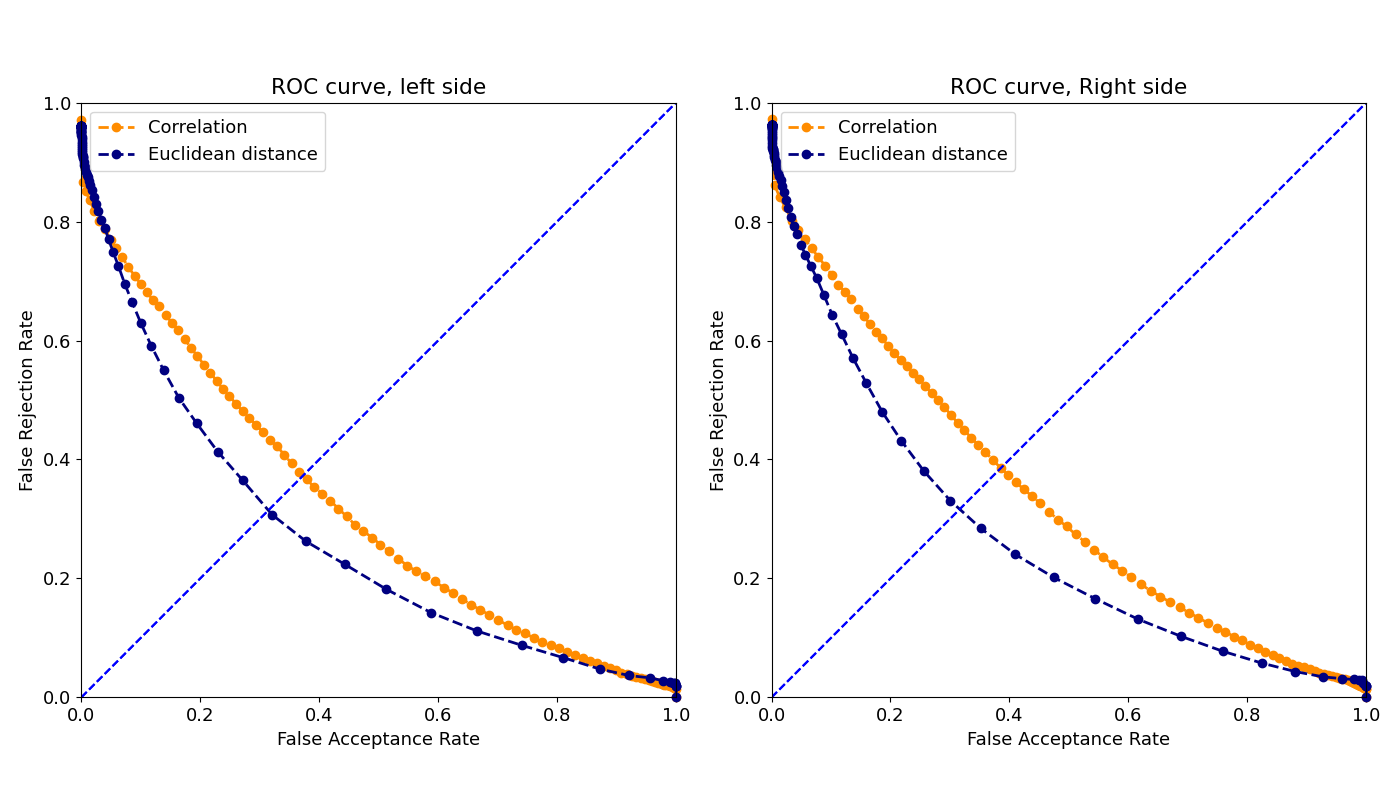
\includegraphics[scale=0.3]{Manuscripts/src/figures/Correlation.png}
\end{frame}

%%%%%%%%%%%%%%%%%%%%%%%%%%%%%%%%%%%%%%%%%%%
%%%%%%%%%%%%%%%%%%%%%%%%%%%%%%%%%%%%%%%%%%%
\section{Criteria}

\begin{frame}
\frametitle{Minimum vs Median vs Average}
\tiny
\begin{table}
\centering
\captionsetup{labelformat=empty}
\caption{\small The accuracy of Minimum, Median and Average.}
\label{tab:parameters condition}
\begin{tabular}{lrrrr}
\toprule
{} &  Accuracy Left &  Accuracy Right &  EER Left &  EER Right \\
\midrule
mean   &          96.46 &           96.37 &      0.30 &       0.30 \\
min    &          73.67 &           70.66 &      0.26 &       0.25 \\
max    &          98.87 &           98.94 &      0.49 &       0.49 \\
median &          98.86 &           98.93 &      0.27 &       0.27 \\
\bottomrule
\end{tabular}

\end{table}
\begin{table}
\centering
\captionsetup{labelformat=empty}
\caption{\small The ERR of Minimum, Median and Average.}
\label{tab:parameters condition}
\begin{tabular}{lll}
\toprule
{} &                    EER Left &                   EER Right \\
\midrule
Minimum &  0.30 +/- 0.06 (0.14, 0.39) &  0.30 +/- 0.06 (0.15, 0.40) \\
Median  &  0.25 +/- 0.09 (0.00, 0.33) &  0.26 +/- 0.09 (0.01, 0.34) \\
Average &  0.36 +/- 0.10 (0.28, 0.75) &  0.35 +/- 0.10 (0.28, 0.72) \\
\bottomrule
\end{tabular}

\end{table}
\end{frame}


\begin{frame}
\centering
\frametitle{Minimum vs Median vs Average (ROC curve)}
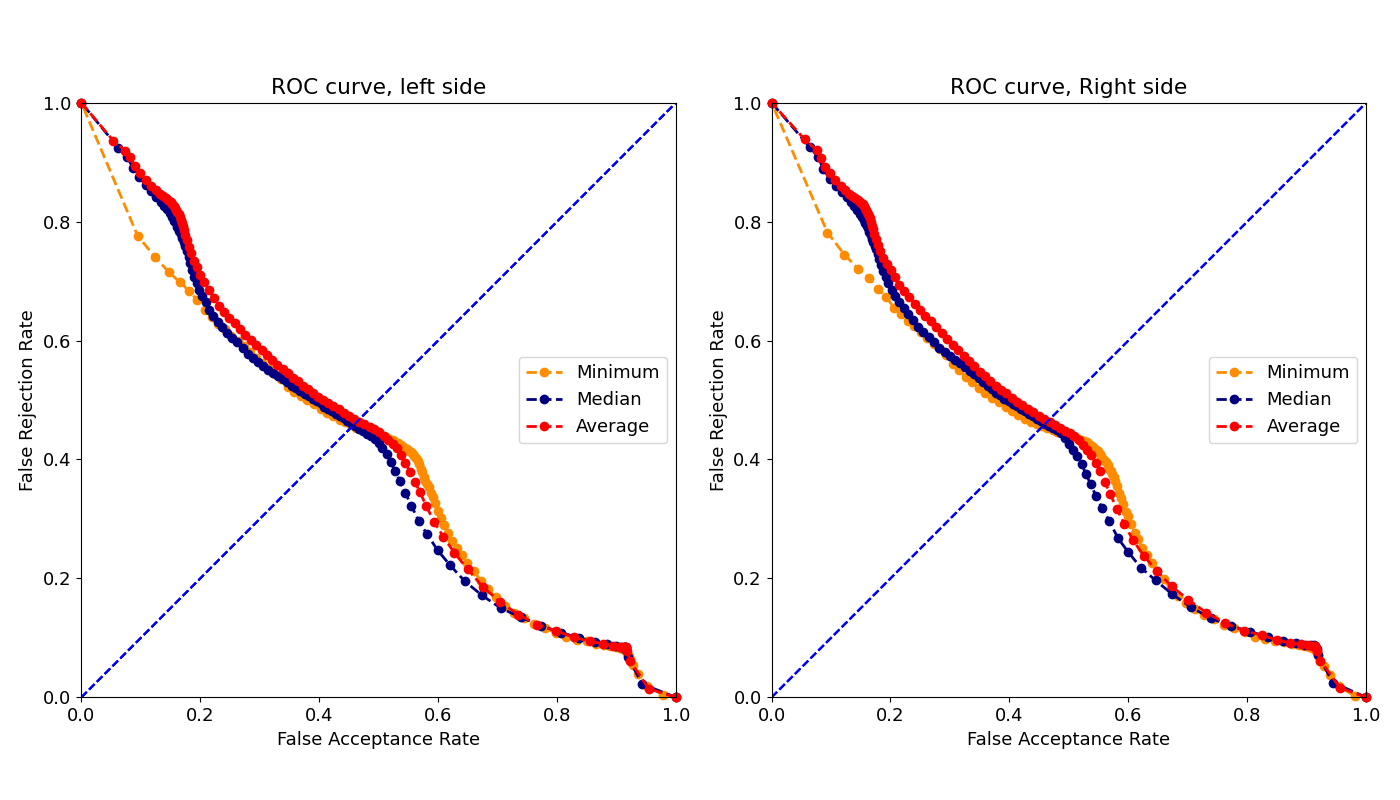
\includegraphics[scale=0.3]{Manuscripts/src/figures/Minimum.png}
\end{frame}


%%%%%%%%%%%%%%%%%%%%%%%%%%%%%%%%%%%%%%%%%%%
%%%%%%%%%%%%%%%%%%%%%%%%%%%%%%%%%%%%%%%%%%%
\section{PCA}

\begin{frame}
\frametitle{All PCs vs Keeping 95 percent of variance}
\tiny
\begin{table}
\centering
\captionsetup{labelformat=empty}
\caption{\small The accuracy of All PCs and Keeping 95 percent of variance.}
\label{tab:parameters condition}
\begin{tabular}{lll}
\toprule
{} &                  Accuracy Left &                 Accuracy Right \\
\midrule
All PCs                        &  64.66 +/- 5.97 (50.00, 77.44) &  63.95 +/- 5.92 (50.69, 74.28) \\
Keeping 95 percent of variance &                            NaN &                            NaN \\
\bottomrule
\end{tabular}

\end{table}
\begin{table}
\centering
\captionsetup{labelformat=empty}
\caption{\small The ERR of All PCs and Keeping 95 percent of variance.}
\label{tab:parameters condition}
\begin{tabular}{lll}
\toprule
{} &                    EER Left &                   EER Right \\
\midrule
All PCs                        &      nan +/- nan (nan, nan) &      nan +/- nan (nan, nan) \\
Keeping 95 percent of variance &  0.20 +/- 0.02 (0.16, 0.21) &  0.21 +/- 0.02 (0.19, 0.23) \\
\bottomrule
\end{tabular}

\end{table}
\end{frame}


\begin{frame}
\centering
\frametitle{All PCs vs Keeping 95 percent of variance (ROC curve)}
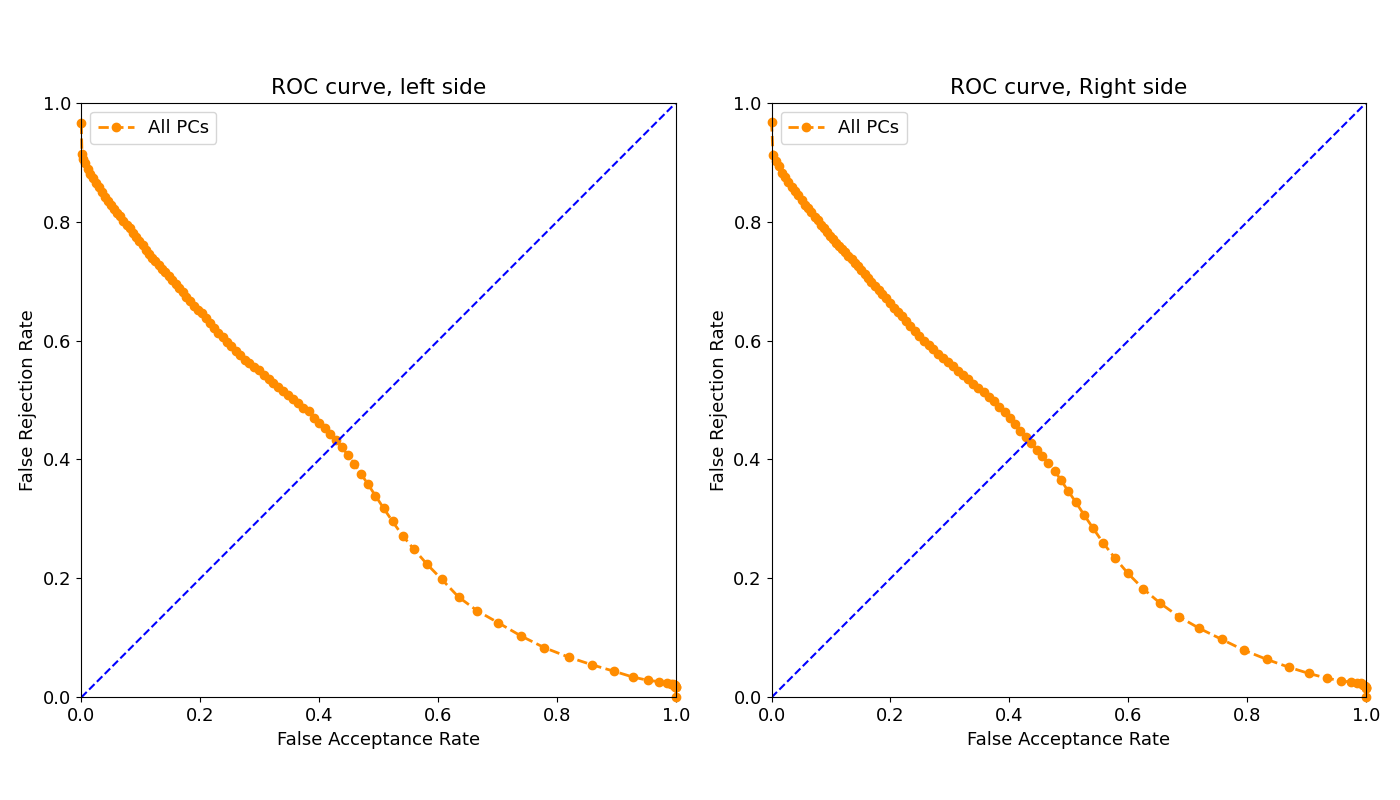
\includegraphics[scale=0.3]{Manuscripts/src/figures/PCA.png}
\end{frame}





%%%%%%%%%%%%%%%%%%%%%%%%%%%%%%%%%%%%%%%%%%%
%%%%%%%%%%%%%%%%%%%%%%%%%%%%%%%%%%%%%%%%%%%
\section{Normalization algorithm}
\def \variable {MinMax}%MinMax

\begin{frame}
\frametitle{Z-score algorithm vs MinMax algorithm vs None}
\tiny
\begin{table}
\centering
\captionsetup{labelformat=empty}
\caption{\small The accuracy of different normalization algorithm.}
\label{tab:parameters condition}
\begin{tabular}{lll}
\toprule
{} &                  Accuracy Left &                 Accuracy Right \\
\midrule
Z-score algorithm &  81.14 +/- 2.47 (78.10, 84.42) &  79.74 +/- 5.19 (71.08, 85.15) \\
MinMax algorithm  &         nan +/- nan (nan, nan) &         nan +/- nan (nan, nan) \\
None              &         nan +/- nan (nan, nan) &         nan +/- nan (nan, nan) \\
\bottomrule
\end{tabular}

\end{table}
\begin{table}
\centering
\captionsetup{labelformat=empty}
\caption{\small The ERR of different normalization algorithm.}
\label{tab:parameters condition}
\begin{tabular}{lll}
\toprule
{} &                    EER Left &                   EER Right \\
\midrule
Z-score algorithm &  0.30 +/- 0.10 (0.00, 0.75) &  0.30 +/- 0.10 (0.01, 0.72) \\
MinMax algorithm  &                         NaN &                         NaN \\
None              &                         NaN &                         NaN \\
\bottomrule
\end{tabular}

\end{table}
\end{frame}


\begin{frame}
\centering
\frametitle{Z-score algorithm vs MinMax algorithm vs None (ROC curve)}
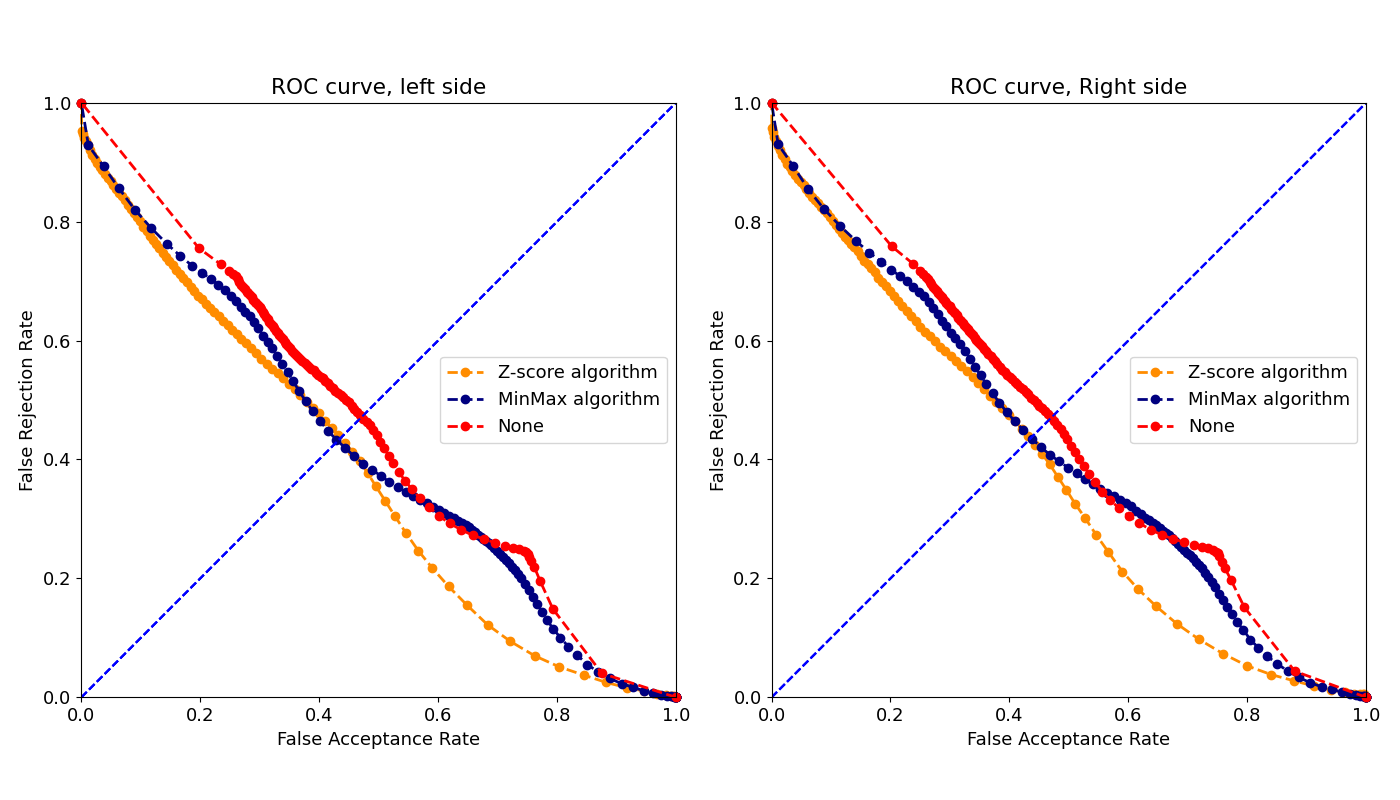
\includegraphics[scale=0.3]{Manuscripts/src/figures/MinMax.png}
\end{frame}




%%%%%%%%%%%%%%%%%%%%%%%%%%%%%%%%%%%%%%%%%%%
%%%%%%%%%%%%%%%%%%%%%%%%%%%%%%%%%%%%%%%%%%%
\section{COP features}


\begin{frame}
\frametitle{Comparing COP features}
\tiny
\begin{table}
\centering
\captionsetup{labelformat=empty}
\caption{\small The accuracy of COP features.}
\label{tab:parameters condition}
\begin{tabular}{lll}
\toprule
{} &                   Accuracy Left &                  Accuracy Right \\
\midrule
All features         &  74.15 +/- 20.00 (26.07, 98.96) &  73.16 +/- 21.22 (23.53, 98.96) \\
Only MDIST features  &   51.18 +/- 36.12 (1.05, 98.96) &   51.38 +/- 35.35 (1.91, 98.96) \\
Only RDIST features  &   50.21 +/- 37.25 (1.06, 98.96) &   50.69 +/- 36.01 (1.86, 98.96) \\
Only TOTEX features  &   55.85 +/- 34.29 (1.66, 98.96) &   56.30 +/- 32.84 (3.05, 98.96) \\
Only MVELO features  &   55.85 +/- 34.29 (1.66, 98.96) &   56.30 +/- 32.84 (3.05, 98.96) \\
Only RANGE features  &   73.53 +/- 34.97 (1.04, 98.96) &   73.54 +/- 34.98 (1.04, 98.96) \\
Only AREAXX features &  71.05 +/- 21.48 (27.95, 98.96) &  68.95 +/- 22.76 (24.81, 98.96) \\
Only MFREQ features  &  64.25 +/- 25.53 (12.84, 98.96) &  64.48 +/- 25.18 (15.22, 98.96) \\
Only FDPD features   &  61.16 +/- 26.57 (12.17, 98.96) &  60.79 +/- 26.15 (13.84, 98.96) \\
Only FDCX features   &   70.38 +/- 35.49 (1.04, 98.96) &   69.61 +/- 35.63 (1.04, 98.96) \\
\bottomrule
\end{tabular}

\end{table}
\end{frame}

\begin{frame}
\frametitle{Comparing COP features}
\tiny
\begin{table}
\centering
\captionsetup{labelformat=empty}
\caption{\small The ERR of COP features.}
\label{tab:parameters condition}
\begin{tabular}{lll}
\toprule
{} &                    EER Left &                   EER Right \\
\midrule
All features         &  0.31 +/- 0.09 (0.01, 0.63) &  0.30 +/- 0.09 (0.01, 0.63) \\
Only MDIST features  &  0.36 +/- 0.12 (0.00, 0.78) &  0.36 +/- 0.11 (0.01, 0.75) \\
Only RDIST features  &  0.35 +/- 0.11 (0.00, 0.76) &  0.34 +/- 0.11 (0.01, 0.71) \\
Only TOTEX features  &  0.36 +/- 0.12 (0.00, 0.75) &  0.35 +/- 0.11 (0.01, 0.74) \\
Only MVELO features  &  0.36 +/- 0.11 (0.00, 0.75) &  0.35 +/- 0.11 (0.01, 0.74) \\
Only RANGE features  &  0.34 +/- 0.10 (0.00, 0.74) &  0.34 +/- 0.10 (0.00, 0.70) \\
Only AREAXX features &  0.37 +/- 0.11 (0.00, 0.77) &  0.37 +/- 0.11 (0.01, 0.76) \\
Only MFREQ features  &  0.40 +/- 0.11 (0.00, 0.82) &  0.38 +/- 0.11 (0.00, 0.76) \\
Only FDPD features   &  0.42 +/- 0.11 (0.00, 0.82) &  0.42 +/- 0.11 (0.01, 0.79) \\
Only FDCX features   &  0.40 +/- 0.21 (0.00, 0.85) &  0.40 +/- 0.21 (0.01, 0.86) \\
\bottomrule
\end{tabular}

\end{table}
\end{frame}


\begin{frame}
\centering
\frametitle{Comparing COP features (ROC curve)}
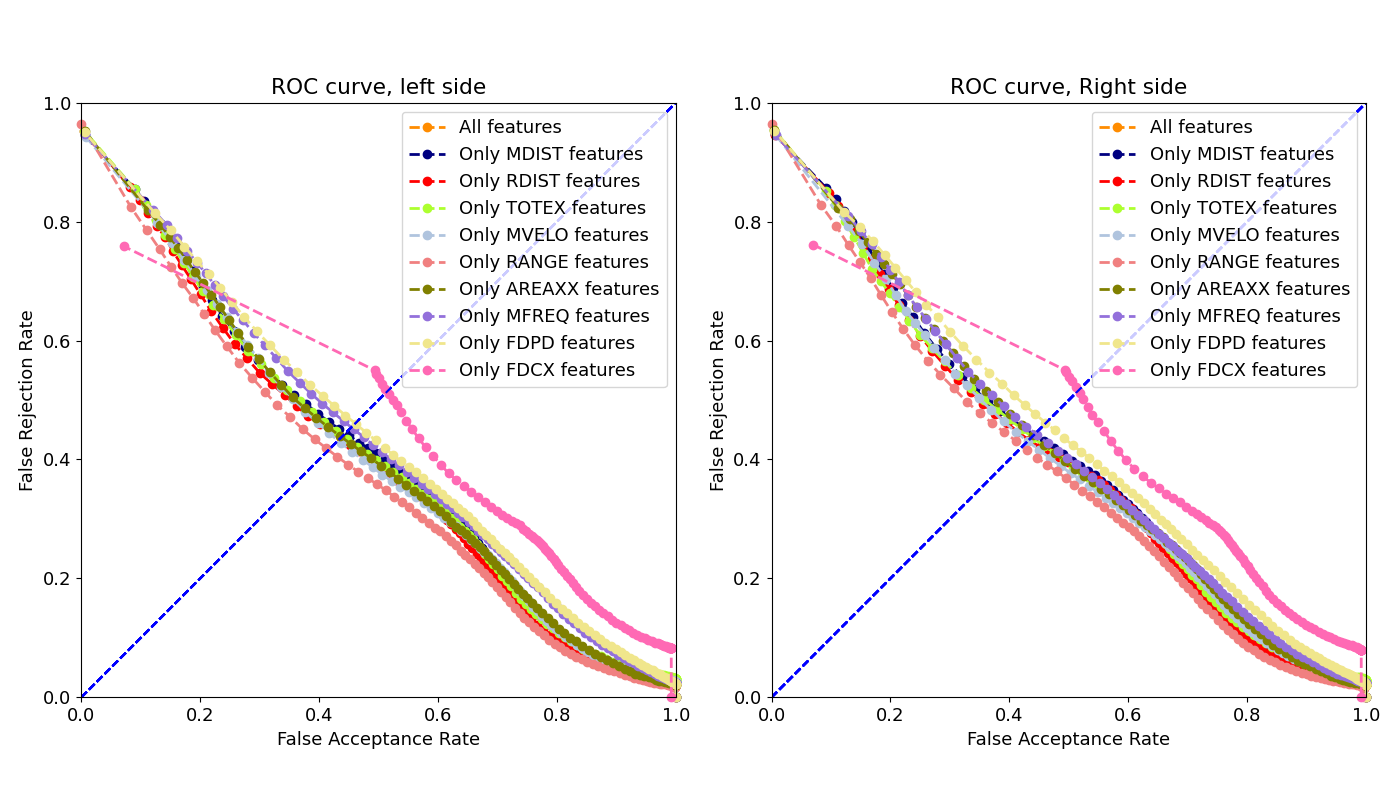
\includegraphics[scale=0.3]{Manuscripts/src/figures/feat.png}
\end{frame}




%%%%%%%%%%%%%%%%%%%%%%%%%%%%%%%%%%%%%%%%%%%
%%%%%%%%%%%%%%%%%%%%%%%%%%%%%%%%%%%%%%%%%%%
\section{The top-10 best and worst features}

\begin{frame}[shrink=10]
\frametitle{The top-10 best features for the left foot.}
\tiny
\begin{table}
\centering
\caption{\small The top-10 best features for the left foot.}
\begin{tabular}{lllrllrrr}
\toprule
{} &  Mode & Model\_Type &  TestSize &     Norm & Features\_Set &   PCA &  Acc\_Left &  EER\_Left \\
index &       &            &           &          &              &       &           &           \\
\midrule
832   &  corr &     median &       0.2 &  z-score &       AREAXX &  0.95 &     98.96 &      0.05 \\
1012  &  corr &     median &       0.2 &   minmax &       AREAXX &  0.95 &     98.96 &      0.05 \\
652   &  corr &     median &       0.2 &     None &       AREAXX &  0.95 &     98.96 &      0.05 \\
526   &  corr &     median &       0.2 &   minmax &         FDCX &  1.00 &     98.96 &      0.06 \\
688   &  corr &     median &       0.2 &     None &         FDPD &  0.95 &     98.96 &      0.06 \\
94    &  corr &     median &       0.2 &     None &        RANGE &  1.00 &     98.96 &      0.06 \\
1048  &  corr &     median &       0.2 &   minmax &         FDPD &  0.95 &     98.96 &      0.06 \\
454   &  corr &     median &       0.2 &   minmax &        RANGE &  1.00 &     98.96 &      0.06 \\
346   &  corr &     median &       0.2 &  z-score &         FDCX &  1.00 &     98.96 &      0.06 \\
868   &  corr &     median &       0.2 &  z-score &         FDPD &  0.95 &     98.96 &      0.07 \\
\bottomrule
\end{tabular}

\end{table}
\end{frame}

%%%%%%%%%%%%%%%%%%%%%%%%%%%%%%%%%%%%%%%%%%%
%%%%%%%%%%%%%%%%%%%%%%%%%%%%%%%%%%%%%%%%%%%
\begin{frame}[shrink=10]
\frametitle{The top-10 best features for the right foot.}
\tiny
\begin{table}
\centering
\caption{\small The top-10 best features for the right foot.}
\begin{tabular}{lllrllrrr}
\toprule
{} &  Mode & Model\_Type &  Test\_Size & Normalizition & Features\_Set &   PCA &  Mean\_Accuracy\_Right &  Mean\_EER\_Right \\
index &       &            &            &               &              &       &                      &                 \\
\midrule
346   &  corr &     median &        0.2 &       z-score &         FDCX &  1.00 &                98.96 &            0.05 \\
94    &  corr &     median &        0.2 &          None &        RANGE &  1.00 &                98.96 &            0.05 \\
832   &  corr &     median &        0.2 &       z-score &       AREAXX &  0.95 &                98.96 &            0.05 \\
652   &  corr &     median &        0.2 &          None &       AREAXX &  0.95 &                98.96 &            0.05 \\
1012  &  corr &     median &        0.2 &        minmax &       AREAXX &  0.95 &                98.96 &            0.05 \\
526   &  corr &     median &        0.2 &        minmax &         FDCX &  1.00 &                98.96 &            0.05 \\
688   &  corr &     median &        0.2 &          None &         FDPD &  0.95 &                98.96 &            0.05 \\
1048  &  corr &     median &        0.2 &        minmax &         FDPD &  0.95 &                98.96 &            0.06 \\
454   &  corr &     median &        0.2 &        minmax &        RANGE &  1.00 &                98.96 &            0.06 \\
868   &  corr &     median &        0.2 &       z-score &         FDPD &  0.95 &                98.96 &            0.06 \\
\bottomrule
\end{tabular}

\end{table}
\end{frame}

%%%%%%%%%%%%%%%%%%%%%%%%%%%%%%%%%%%%%%%%%%%
%%%%%%%%%%%%%%%%%%%%%%%%%%%%%%%%%%%%%%%%%%%
\begin{frame}[shrink=10]
\frametitle{The top-10 worst features for the left foot.}
\tiny
\begin{table}
\centering
\caption{\small The top-10 worst features for the left foot.}
\begin{tabular}{lllrllrrr}
\toprule
{} &  Mode & Model\_Type &  Test\_Size & Normalizition & Features\_Set &   PCA &  Mean\_Accuracy\_Left &  Mean\_EER\_Left \\
index &       &            &            &               &              &       &                     &                \\
\midrule
655   &  corr &    average &        0.2 &          None &       AREAXX &  0.95 &                1.04 &           0.67 \\
529   &  corr &    average &        0.2 &        minmax &         FDCX &  1.00 &                1.04 &           0.66 \\
1015  &  corr &    average &        0.2 &        minmax &       AREAXX &  0.95 &                1.04 &           0.66 \\
835   &  corr &    average &        0.2 &       z-score &       AREAXX &  0.95 &                1.04 &           0.66 \\
691   &  corr &    average &        0.2 &          None &         FDPD &  0.95 &                1.04 &           0.66 \\
1051  &  corr &    average &        0.2 &        minmax &         FDPD &  0.95 &                1.04 &           0.65 \\
871   &  corr &    average &        0.2 &       z-score &         FDPD &  0.95 &                1.04 &           0.64 \\
457   &  corr &    average &        0.2 &        minmax &        RANGE &  1.00 &                1.04 &           0.64 \\
349   &  corr &    average &        0.2 &       z-score &         FDCX &  1.00 &                1.04 &           0.62 \\
277   &  corr &    average &        0.2 &       z-score &        RANGE &  1.00 &                1.04 &           0.62 \\
\bottomrule
\end{tabular}

\end{table}
\end{frame}

%%%%%%%%%%%%%%%%%%%%%%%%%%%%%%%%%%%%%%%%%%%
%%%%%%%%%%%%%%%%%%%%%%%%%%%%%%%%%%%%%%%%%%%
\begin{frame}[shrink=10]
\frametitle{The top-10 worst features for the right foot.}
\tiny
\begin{table}
\centering
\caption{\small The top-10 worst features for the right foot.}
\begin{tabular}{lllrllrrr}
\toprule
{} &  Mode & Model\_Type &  TestSize &     Norm & Features\_Set &   PCA &  Acc\_Right &  EER\_Right \\
index &       &            &           &          &              &       &            &            \\
\midrule
529   &  corr &    average &       0.2 &   minmax &         FDCX &  1.00 &       1.04 &       0.67 \\
655   &  corr &    average &       0.2 &     None &       AREAXX &  0.95 &       1.04 &       0.67 \\
1015  &  corr &    average &       0.2 &   minmax &       AREAXX &  0.95 &       1.04 &       0.66 \\
835   &  corr &    average &       0.2 &  z-score &       AREAXX &  0.95 &       1.04 &       0.66 \\
691   &  corr &    average &       0.2 &     None &         FDPD &  0.95 &       1.04 &       0.65 \\
871   &  corr &    average &       0.2 &  z-score &         FDPD &  0.95 &       1.04 &       0.65 \\
1051  &  corr &    average &       0.2 &   minmax &         FDPD &  0.95 &       1.04 &       0.65 \\
349   &  corr &    average &       0.2 &  z-score &         FDCX &  1.00 &       1.04 &       0.63 \\
457   &  corr &    average &       0.2 &   minmax &        RANGE &  1.00 &       1.04 &       0.63 \\
169   &  corr &    average &       0.2 &     None &         FDCX &  1.00 &       1.04 &       0.63 \\
\bottomrule
\end{tabular}

\end{table}
\end{frame}


%%%%%%%%%%%%%%%%%%%%%%%%%%%%%%%%%%%%%%%%%%%
%%%%%%%%%%%%%%%%%%%%%%%%%%%%%%%%%%%%%%%%%%%
\section{Feature Selection Results}
\begin{frame}[shrink=10]
\frametitle{The top-10 best features based on feature selection algorithm.}
\tiny
\begin{table}
\centering
\caption{\small The top-10 best features based on feature selection algorithm.}
\begin{tabular}{llllll}
\toprule
{} &     D-prime &     F-ratio &    mRMR-Dif &      mRMR-Q &  Redundancy \\
\midrule
0 &  feature\_20 &   feature\_0 &  feature\_20 &  feature\_20 &   feature\_3 \\
1 &  feature\_16 &   feature\_7 &  feature\_25 &  feature\_25 &   feature\_9 \\
2 &  feature\_25 &  feature\_10 &  feature\_16 &  feature\_18 &   feature\_6 \\
3 &   feature\_0 &  feature\_13 &  feature\_18 &  feature\_21 &  feature\_15 \\
4 &  feature\_18 &  feature\_12 &  feature\_21 &  feature\_16 &   feature\_4 \\
5 &  feature\_21 &   feature\_1 &   feature\_0 &  feature\_22 &   feature\_0 \\
6 &   feature\_1 &  feature\_16 &   feature\_2 &   feature\_2 &  feature\_13 \\
7 &   feature\_2 &  feature\_20 &   feature\_1 &   feature\_0 &  feature\_12 \\
8 &   feature\_7 &  feature\_18 &  feature\_24 &   feature\_1 &   feature\_7 \\
9 &  feature\_10 &  feature\_25 &   feature\_5 &  feature\_24 &  feature\_10 \\
\bottomrule
\end{tabular}

\end{table}
\end{frame}

%%%%%%%%%%%%%%%%%%%%%%%%%%%%%%%%%%%%%%%%%%%
%%%%%%%%%%%%%%%%%%%%%%%%%%%%%%%%%%%%%%%%%%%
\begin{frame}[shrink=10]
\frametitle{The top-10 worst features based on feature selection algorithm.}
\tiny
\begin{table}
\centering
\caption{\small The top-10 worst features based on feature selection algorithm.}
\begin{tabular}{llllll}
\toprule
{} &     D-prime &     F-ratio &    mRMR-Dif &      mRMR-Q &  Redundancy \\
\midrule
16 &   feature\_8 &  feature\_22 &  feature\_11 &   feature\_8 &   feature\_2 \\
17 &  feature\_19 &   feature\_5 &   feature\_8 &  feature\_11 &  feature\_14 \\
18 &   feature\_4 &  feature\_19 &  feature\_23 &   feature\_3 &  feature\_21 \\
19 &  feature\_15 &  feature\_11 &   feature\_3 &   feature\_4 &  feature\_24 \\
20 &  feature\_14 &   feature\_8 &  feature\_14 &  feature\_14 &  feature\_18 \\
21 &  feature\_22 &  feature\_14 &   feature\_4 &  feature\_15 &  feature\_19 \\
22 &  feature\_17 &  feature\_17 &  feature\_15 &  feature\_23 &  feature\_25 \\
23 &  feature\_23 &   feature\_9 &  feature\_17 &  feature\_17 &  feature\_20 \\
24 &   feature\_9 &   feature\_6 &   feature\_6 &   feature\_6 &  feature\_23 \\
25 &   feature\_6 &  feature\_23 &   feature\_9 &   feature\_9 &  feature\_22 \\
\bottomrule
\end{tabular}

\end{table}
\end{frame}


%%%%%%%%%%%%%%%%%%%%%%%%%%%%%%%%%%%%%%%%%%%
%%%%%%%%%%%%%%%%%%%%%%%%%%%%%%%%%%%%%%%%%%%
\begin{frame}
\frametitle{The feature correlation plot.}
\centering
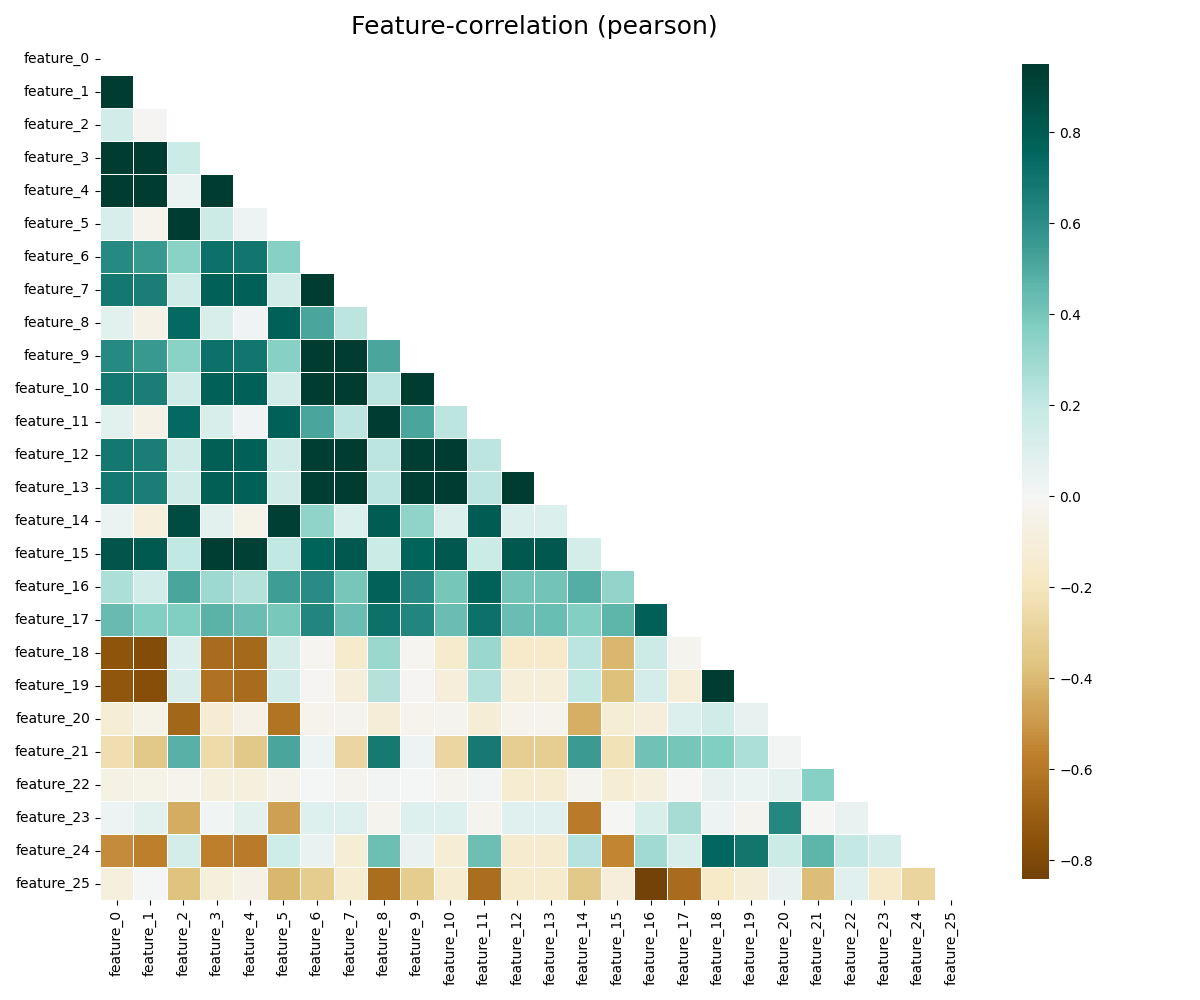
\includegraphics[scale=0.3]{Manuscripts/src/figures/corr_plot.png}
\end{frame}

%%%%%%%%%%%%%%%%%%%%%%%%%%%%%%%%%%%%%%%%%%%
%%%%%%%%%%%%%%%%%%%%%%%%%%%%%%%%%%%%%%%%%%%
%\section{Summary}

%\begin{frame}{Summary}

%\begin{itemize}
%    \item gg
%\end{itemize}

    
%\end{frame}

%%%%%%%%%%%%%%%%%%%%%%%%%%%%%%%%%%%%%%%%%%%
%%%%%%%%%%%%%%%%%%%%%%%%%%%%%%%%%%%%%%%%%%%


%%%%%%%%%%%%%%%%%%%%%%%%%%%%%%%%%%%%%%%%%%%
%%%%%%%%%%%%%%%%%%%%%%%%%%%%%%%%%%%%%%%%%%%

\end{document}

